\chapter{Background}
\label{chap:background}

% A more extensive coverage of what's required to understand your work.
% In general you should assume the reader has a good undergraduate
% degree in computer science, but is not necessarily an expert in the
% particular area you've been working on. Hence this chapter may need to
% summarize some ``text book'' material.
%
% This is not something you'd normally require in an academic paper, and
% it may not be appropriate for your particular circumstances. Indeed,
% in some cases it's possible to cover all of the ``background''
% material either in the introduction or at appropriate places in the
% rest of the dissertation.



\begin{figure}[H]
    \centering
    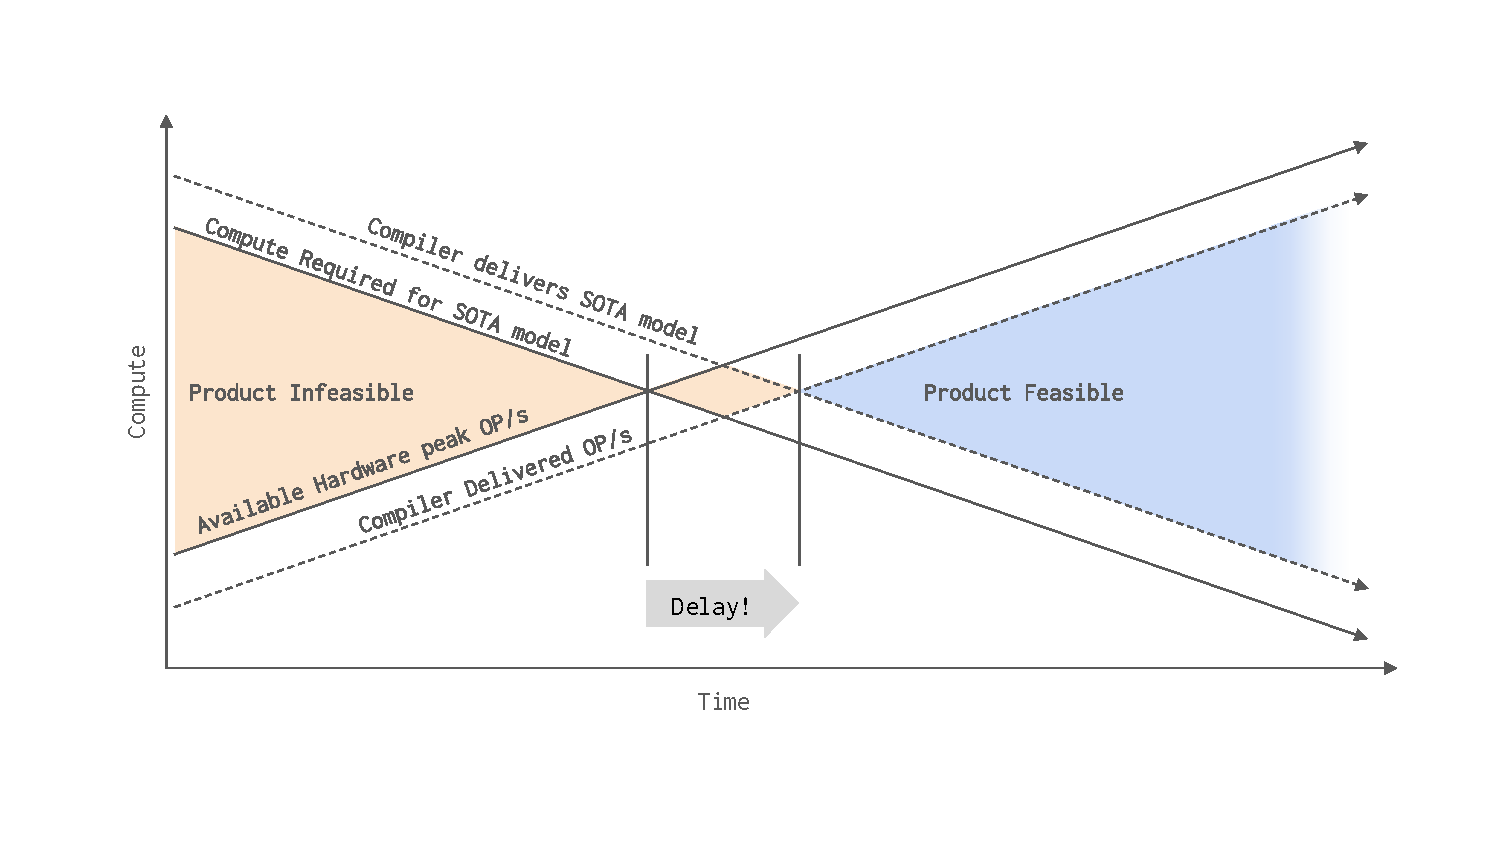
\includegraphics[width=\textwidth]{images/11_introduction/compilers_lagging.pdf}
    \caption{Compilers are lagging behind the development of both machine learning hardware and workloads. Figure created by Anton Lydike based on a slide from Sean Silva's talk at the March 2025 Cambridge Compiler Social.}
    \label{fig:compilers-lagging}
\end{figure}



% \section{Compilation}
% \label{sec:compilation}

% \section{LLVM and SSA}
% \label{sec:llvm-ssa}

% \section{MLIR}
% \label{sec:mlir}

% \section{IRDL and PDL}
% \label{sec:irdl}

% \section{xDSL}
% \label{sec:xdsl}




% \section{Python internals}
% \label{sec:python-internals}

% A brief overview of how Python works, talking about bytecode and stuff


% \section{Python performance}
% \label{sec:python-performance}

% % \subsection{Python performance matters}
% % \label{ssec:python-performance-matters}

% Typically, we want to bind into C as much as possible -- see things like Scalene to measure this. However, for our pattern rewriting workload, this is less suitable

% \subsection{Python performance measurement}
% \label{ssec:python-perf-measurement}
% timeit/asv/pyperf and stuff maybe? Possibly not worth discussing

